\documentclass[fullscreen=true, bookmarks=true, hyperref={pdfencoding=unicode}]{beamer}
\usepackage[utf8]{inputenc}                                % Кодировка
\usepackage[english,russian]{babel}                        % Переносы
\usepackage{xcolor}                                        % Работа с цветом
\usepackage{amsmath,amssymb,amsfonts}                      % Символы АМО
\usepackage{graphicx}                                      % Графика
\usepackage[labelsep=period]{caption}                      % Разделитель в подписях к рисункам и таблицам
\usepackage{hhline}                                        % Для верстки линий в таблицах
\usepackage{tikz}                                          % Для простых рисунков в документе
\usepackage{fancybox}                                      % Пакет для отрисовки рамок
\usepackage{verbatim}                                      % Для вставки кода в презентацию
\usepackage{animate}                                       % Для вставки видео в презентацию
\usepackage{xmpmulti}                                      % Для вставки gif в презентацию
\usepackage{multirow}
\usepackage{mathrsfs}
\usepackage[normalem]{ulem}

\usetikzlibrary{arrows, snakes, backgrounds}                 % Для отрисовки стрелок
\usetikzlibrary{positioning, fit, arrows.meta, shapes, calc}
% used to avoid putting the same thing several times...
% Command \empt{var1}{var2}
\newcommand{\empt}[2]{$#1^{\langle #2 \rangle}$}

\graphicspath{{images/}}                                   % Путь до рисунков
\setbeamertemplate{caption}[numbered]                      % Включение нумерации рисунков

\definecolor{links}{HTML}{2A1B81}                          % blue for url links
\hypersetup{colorlinks,linkcolor=,urlcolor=links}          % nothing for others

\usetheme{boxes}
\usecolortheme{crane}

\usepackage{pythonhighlight}

\newtheorem*{question}{Вопрос}

\title{Лекция 13. Введение в обучение с подкреплением}
\author{Александр Юрьевич Авдюшенко}
\institute{МКН СПбГУ}
\date{12 мая 2022}
\titlegraphic{
\includegraphics[keepaspectratio,width=0.5\textwidth]{logo_fmkn.png}}


\begin{document}
%\unitlength=2mm

% выводим заглавие
\begin{frame}
\transdissolve[duration=0.2]
\titlepage
\end{frame}


\begin{frame}
  \frametitle{Пятиминутка}
  \begin{itemize}
    \item Опишите варианты постановки задачи сегментации изображений
    \item В чем основная идея архитектуры U-net?
    \item Выпишите пару метрик в задаче сегментации
  \end{itemize}
\end{frame}


\begin{frame}
  \frametitle{Обучение с учителем}

  {\bf Дано:}

  Обучающая выборка в виде пар $(x, y)$

  \vspace{1cm}
  Нужно найти $a_\theta(x) \approx y(x)$ в смысле функции потерь $\mathscr{L}(y, a_\theta(x))$

  \pause
  \vspace{1cm}
  \begin{block}{Замечание}
    В реальном мире такого почти никогда нет.
  \end{block}

\end{frame}


\begin{frame}
  \frametitle{Реальный мир}

  \begin{center}
    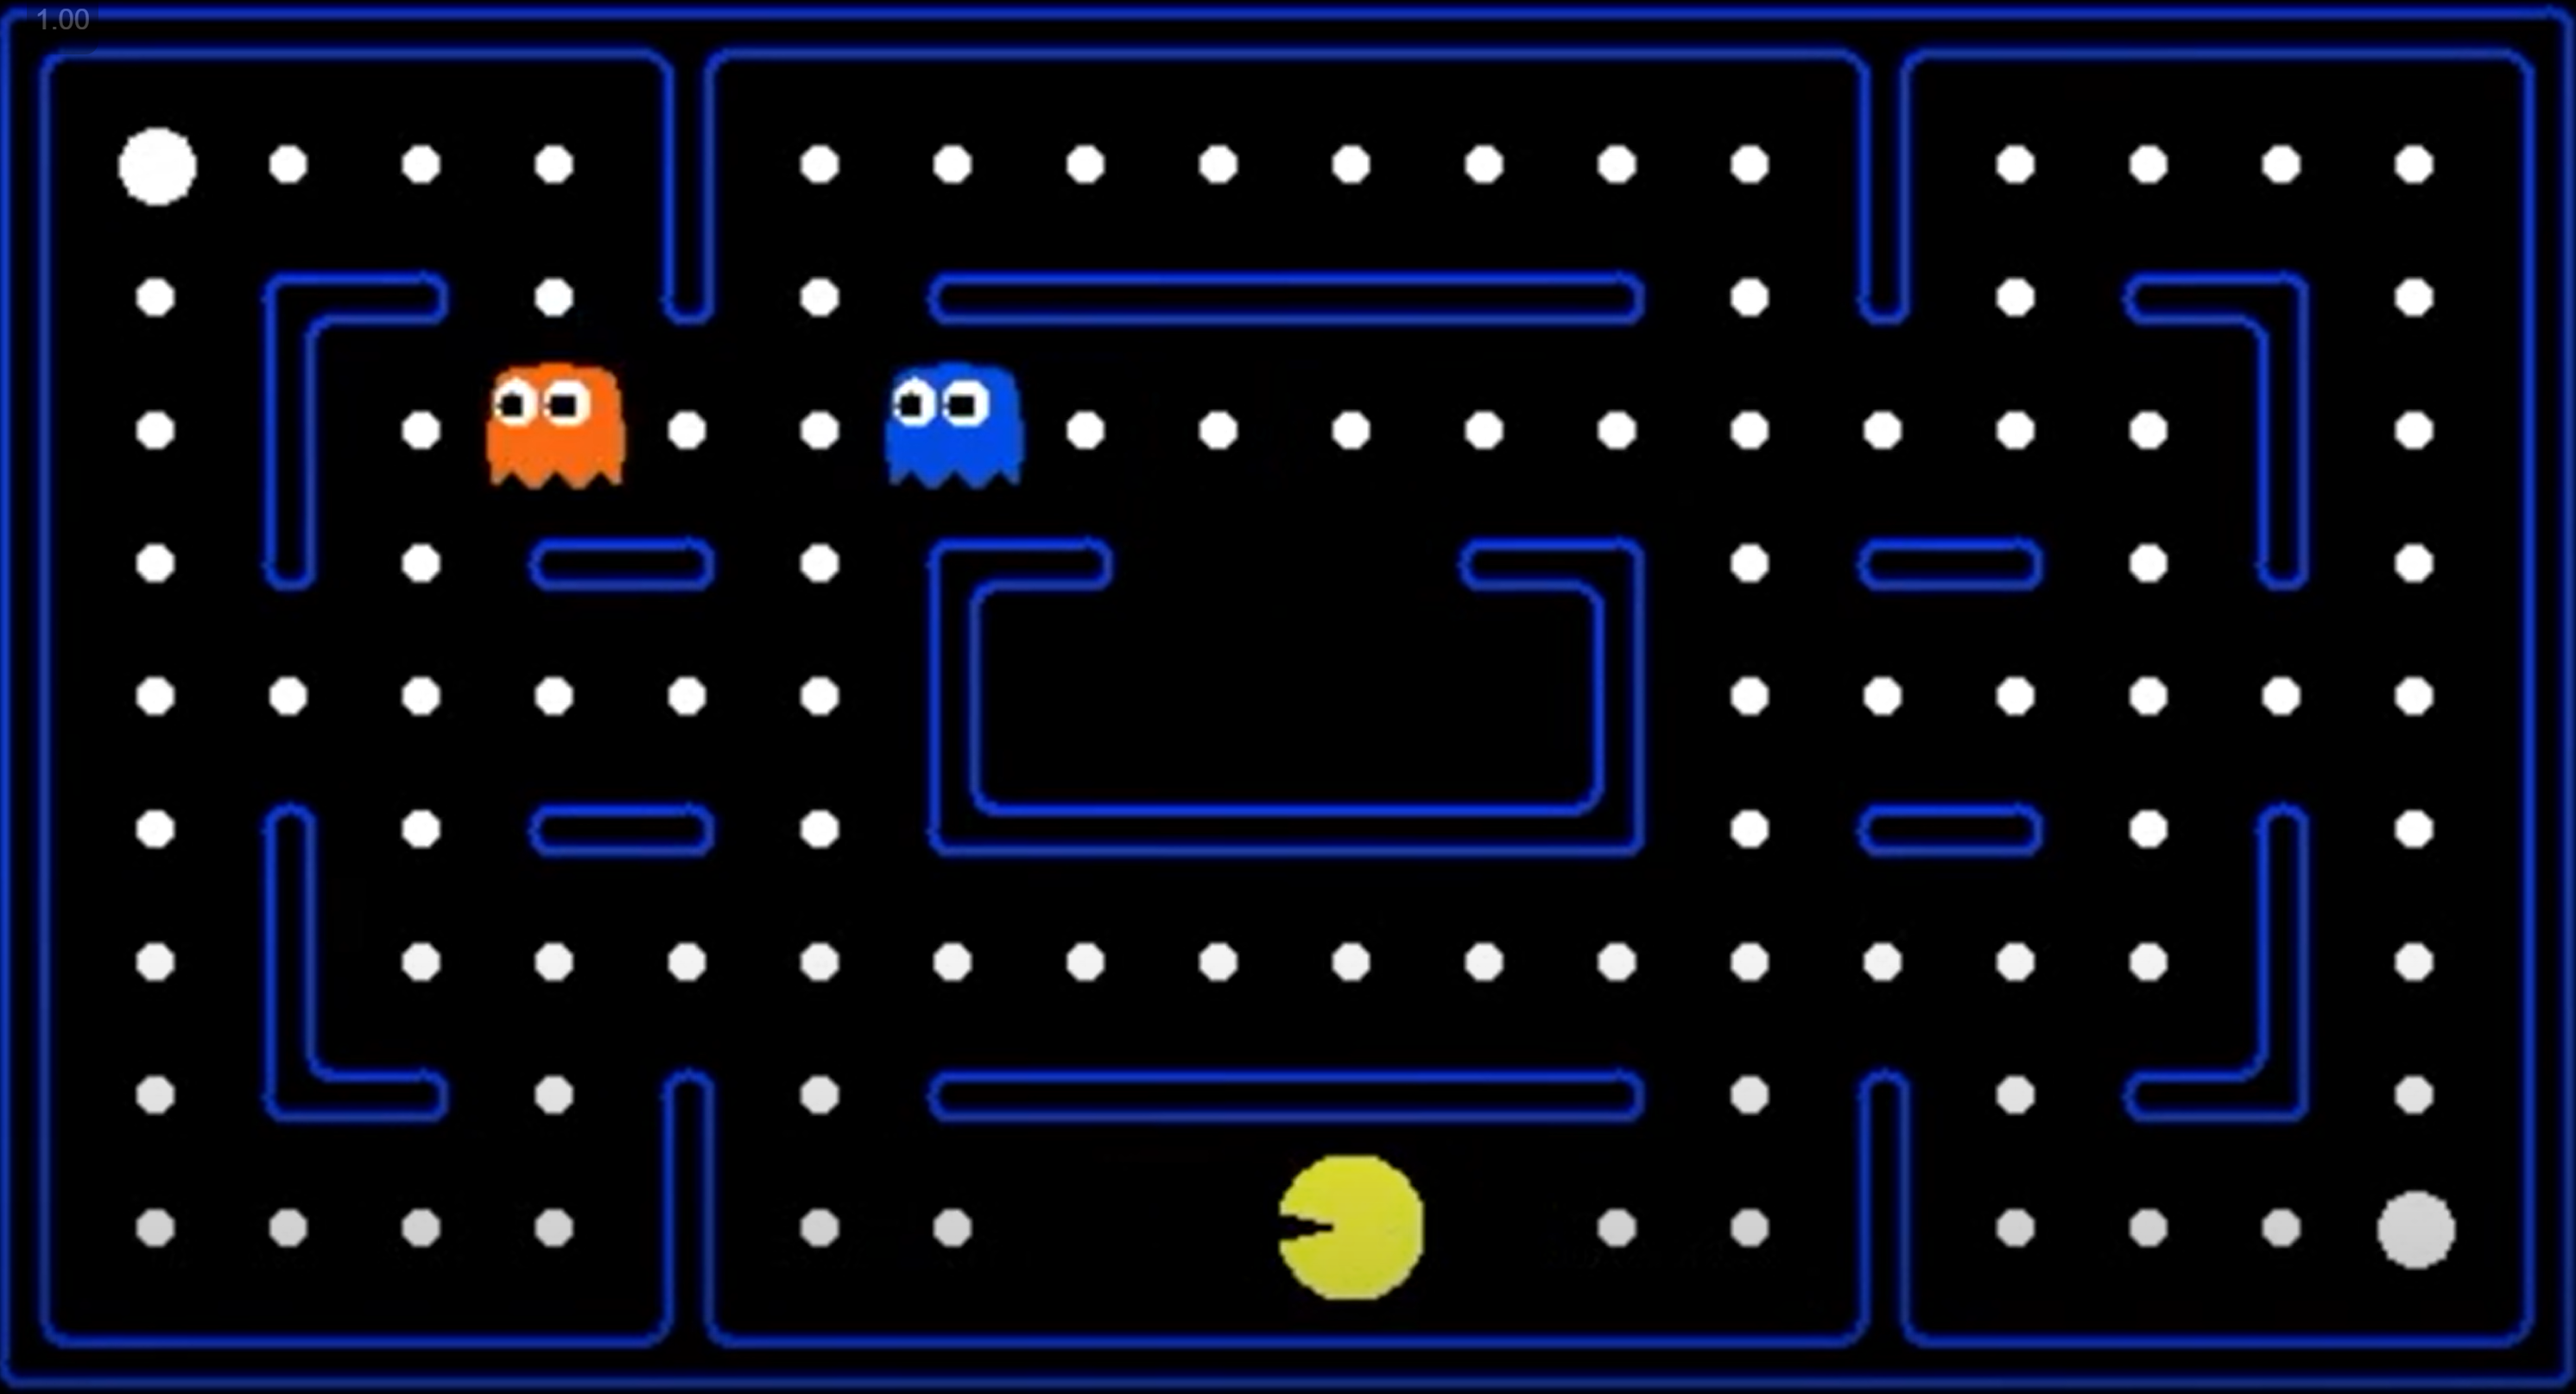
\includegraphics[keepaspectratio,
                     width=.8\paperwidth]{pacman.png}

                     \href{https://www.youtube.com/watch?v=QilHGSYbjDQ}{Deep Reinforcement Learning in Pac-man}
  \end{center}

\end{frame}


\begin{frame}
  \frametitle{Многорукие бандиты}
  \framesubtitle{Напоминание}

  \begin{columns}
    \begin{column}{.4\paperwidth}
      Возможные применения:
      \begin{itemize}
        \item рекламные баннеры
        \item рекомендации (товары, музыка, фильмы, лента)
        \item игровые автоматы
      \end{itemize}
    \end{column}
    \begin{column}{.4\paperwidth}
      Подходы:
      \begin{itemize}
        \item сэмплирование Томпсона
        \item Upper Confidence Bound (UCB)
        \item $\varepsilon$-жадная стратегия
      \end{itemize}
    \end{column}
  \end{columns}

  \vspace{1cm}
  Главное отличие от более общего обучения с подкреплением — в многоруких бандитах нет состояния среды

\end{frame}


\begin{frame}
  \frametitle{Многорукие бандиты}
  \framesubtitle{Недостаток}

  Не учитывают отложенные по времени последствия

  Например, эффект от кликбейта в рекламе

  \pause
  \begin{center}
    
\includegraphics[keepaspectratio,
                     width=.45\paperwidth]{cats_invaders.jpg}

    ШОК! Коты хотят поработить нас
  \end{center}

\end{frame}


\begin{frame}
  \frametitle{Обучение с подкреплением}
  \framesubtitle{Примеры}

  \begin{center}
    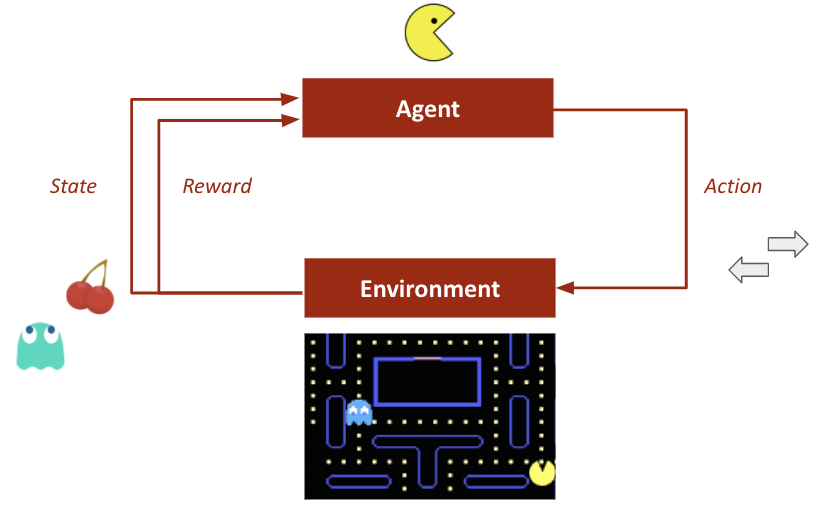
\includegraphics[keepaspectratio,
                     width=.7\paperwidth]{rl_scheme.png}
  \end{center}

  \begin{itemize}
    \item управление роботами
    \item (видео)игры
    \item управление ценными бумагами
  \end{itemize}
\end{frame}


\begin{frame}
  \frametitle{Модель агента в изменяющейся среде}

  \begin{columns}
    \begin{column}{.6\paperwidth}
      {\bf Определения:}
      \begin{itemize}
        \item состояния среды (state) $s \in S$
        \item действия агента (action) $a \in A$
        \item награды (reward) $r \in R$
        \item динамика переходов между состояниями

         $ P(s_{t+1} | s_t, a_t, \dots, s_{t-i}, a_{t-i}, \dots, s_0, a_0) $
        \item функция выигрыша

         $$ r_{t} = r(s_t, a_t, \dots, s_0, a_0)$$
        \item абсолютный выигрыш (total reward)

         $$ R = \sum\limits_t r_t $$
        \item стратегия агента (policy)

         $$ \pi (a | s) $$
      \end{itemize}
    \end{column}
    \begin{column}{.3\paperwidth}
      {\bf Задача:}
      $$ \pi (a | s): \mathbb{E}_\pi [R] \to \max $$
    \end{column}
  \end{columns}

\end{frame}


\begin{frame}
  \frametitle{Метод кросс-энтропии. Алгоритм}

  Траектория — $\left[s_0, a_0, s_1, a_1, s_2, \dots , a_{T-1}, s_T \right]$

  \vspace{1cm}
  {\bf Инициализируем} модель стратегии $\pi(a | s)$

  \vspace{1cm}
  {\bf Повторяем}:
  \begin{itemize}
    \item играем $N$ сессий
    \item выбираем из них $K$ лучших и берем их траектории
    \item настраиваем $\pi(a | s)$ так, чтобы в состоянии $s$ максимизировать вероятности действий из лучших траекторий
  \end{itemize}

\end{frame}


\begin{frame}
  \frametitle{Пример обучения}

  \begin{center}
    \animategraphics[loop,width=0.6\paperwidth,autoplay]{4}{CartPole-v1-}{0}{157}
  \end{center}
\end{frame}


\begin{frame}
  \frametitle{Метод кросс-энтропии. Реализация с помощью таблицы}

  В качестве модели стратегии берем просто матрицу $\pi$ размерности $| S | \times | A |$

  $\pi(a | s) = \pi_{s,a}$

  после отбора лучших траекторий получаем набор пар

  $$\text{Elite} = [(s_0, a_0), (s_1, a_1), (s_2, a_2), \dots, (s_H, a_H )]$$

  и максимизируем правдоподобие

  $$ \pi_{s,a} = \frac{\sum\limits_{s_t, a_t \in \text{Elite}} [s_t = s][a_t = a]}{\sum\limits_{s_t, a_t \in \text{Elite}} [s_t = s]}$$

\end{frame}


\begin{frame}
  \frametitle{Проблема..}

  в том, что состояний очень много:

  \begin{center}
    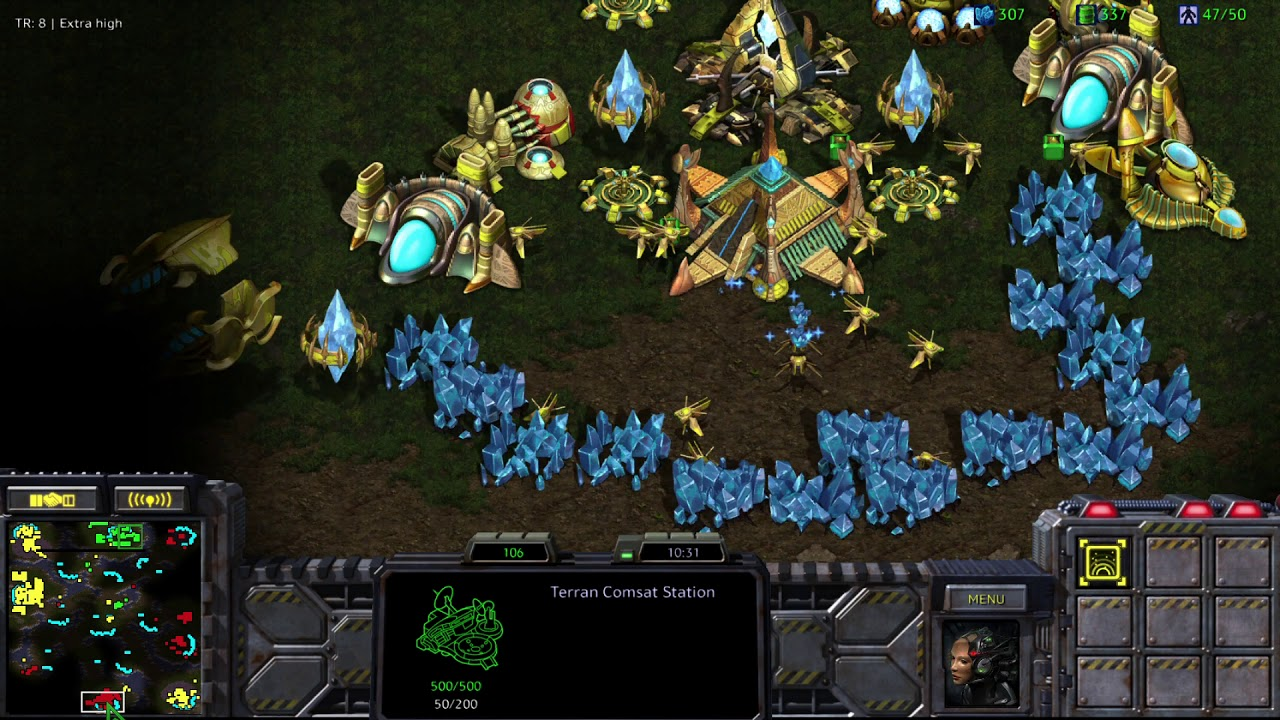
\includegraphics[keepaspectratio,
                     width=.85\paperwidth]{starcraft3.jpg}
  \end{center}
\end{frame}


\begin{frame}
  \frametitle{Аппроксимированный метод кросс-энтропии}

  Возможные решения:
  \begin{itemize}
    \item разбить пространство состояний на участки и считать их состояниями
    \pause
    \item получать вероятности из модели машинного обучения $\pi_\theta (a | s)$: линейная модель, нейронная сеть, случайный лес
    \item часто эти вероятности потом ещё нужно дорабатывать
  \end{itemize}
\end{frame}


\begin{frame}
  \frametitle{Аппроксимированный метод кросс-энтропии}
  \framesubtitle{Пример}

  \begin{itemize}
    \item В качестве модели стратегии берем просто нейронную сеть $\pi_\theta$

    \item Инициализируем случайными весами

    \item На каждой итерации после отбора лучших траекторий получаем набор пар
      $$\text{Elite} = [(s_0, a_0), (s_1, a_1), (s_2, a_2), \dots, (s_H, a_H )]$$

    \item и выполняем оптимизацию
      $$ \pi = \arg\max\limits_\theta \sum\limits_{s_i, a_i \in \text{Elite}} \log \pi(a_i|s_i) = \arg\max\limits_\theta \mathscr{L}(\theta)$$

    \item то есть
      $$ \theta_{t+1} = \theta_{t} + \alpha \nabla \mathscr{L}(\theta) $$
  \end{itemize}
\end{frame}


\begin{frame}
  \frametitle{Почему метод кросс-энтропии?}

  \begin{align*}
    KL(p_1(x) \| p_2(x)) = E_{x \sim p_1(x)} \log \frac{p_1(x)}{p_2(x)} = \\
    =
    \underbrace{E_{x \sim p_1(x)} \log {p_1(x)}}_{
      \text{энтропия}
    } -
    \underbrace{E_{x \sim p_1(x)} \log {p_2(x)}}_{
    \text{кросс-энтропия}
    }
  \end{align*}

\end{frame}


\begin{frame}
  \frametitle{Недостатки метода кросс-энтропии}

  \begin{itemize}
    \item нестабилен при малых выборках
    \item в случае не детерминистской среды выбираем удачные случаи (случайность играла в пользу агента)
    \item концентрируемся на поведении в простых состояниях
    \item игнорируем большое количество информации
    \item есть задачи, в которых конец не настаёт никогда (игра на бирже)
  \end{itemize}
\end{frame}


\begin{frame}
  \frametitle{Q-Learning}

  \begin{itemize}
    \item порой для оценки эффективности стратегии не обязательно доигрывать
    \item эффект от действия может проявиться позднее
  \end{itemize}
\end{frame}


\begin{frame}
  \frametitle{Markov Decision Process}

  \begin{columns}
    \begin{column}{.6\paperwidth}
      {\bf Определения:}
      \begin{itemize}
        \item состояния среды (state) $s \in S$
        \item действия агента (action) $a \in A$
        \item награды (reward) $r \in R$
        \item динамика переходов

         $ P(s_{t+1} | s_t, a_t, \dots, s_{t-i}, a_{t-i}, \dots, s_0, a_0) = P(s_{t+1} | s_t, a_t)$
         {\bf (допущение Маркова)}

        \item функция выигрыша

         $$ r_{t} = r(s_t, a_t)$$ {\bf (допущение Маркова)}
        \item абсолютный выигрыш (total reward)

         $$ R = \sum\limits_t r_t $$
      \end{itemize}
    \end{column}
    \begin{column}{.3\paperwidth}

      \begin{itemize}
        \item стратегия агента (policy)

        $$ \pi (a | s) $$
      \end{itemize}
      {\bf Задача:}
      $$ \pi (a | s): \mathbb{E}_\pi [R] \to \max $$
    \end{column}
  \end{columns}

\end{frame}


\begin{frame}
  \frametitle{Важные функции}
  Средний абсолютный выигрыш:
  $$ \mathbb{E}_{s_0 \sim p(s_0),} \mathbb{E}_{a_0 \sim \pi(a|s_0),} \mathbb{E}_{s_1, r_0 \sim P(s^\prime,r|s, a)} \dots \left[r_0 + r_1 + \dots + r_T \right]$$

  Функция ценности состояния (value function):
  $$ V^{\pi} (s) = \mathbb{E}_\pi [R_t|s_t = s] =
  \mathbb{E}_\pi \left[\sum\limits_{k=0}^\infty \gamma^k r_{t+k+1} | s_t = s \right],$$

  Функция ценности действия в состоянии:
  $$ Q^{\pi} (s, a) = \mathbb{E}_\pi [R_t|s_t = s, a_t = a] =
  \mathbb{E}_\pi \left[\sum\limits_{k=0}^\infty \gamma^k r_{t+k+1} | s_t = s, a_t = a \right],$$

  где $\pi$ — это стратегия, которой следует агент, $\gamma \in [0, 1]$

\end{frame}


\begin{frame}
  \frametitle{TD-обучение}
  \framesubtitle{temporal difference}

  Произвольно инициализируем функцию $V(s)$ и стратегию $\pi$

  Далее повторяем
  \begin{itemize}
    \item инициализируем $s$
    \item для каждого шага агента
      \begin{itemize}
        \item выбрать $a$ по стратегии $\pi$
        \item сделать действие $a$, получить результат $r$ и следующее состояние $s^\prime$
        \item обновить функцию $V(s)$ по формуле
        $$ V(s) = V(s) + \alpha \left(r + \gamma V(s^\prime) - V(s) \right)$$
        \item перейти к следующему шагу, присвоив $s := s^\prime$
      \end{itemize}
  \end{itemize}
\end{frame}


\begin{frame}
  \frametitle{Уравнение Беллмана}
  \framesubtitle{для оптимальной функции ценности $Q^*$}

  $$ Q^* (s,a) = \mathbb{E}_\pi \left[r_t + \gamma \max\limits_{a^\prime} Q^* (s_{t+1},a^\prime) \mid s_t = s, a_t = a \right]$$

  \vspace{1cm}
  \begin{block}{Замечание}
    Жадная стратегия $\pi$ относительно $Q^*(s,a)$ «выбрать то действие, на котором достигается максимум в уравнениях Беллмана», является оптимальной.
  \end{block}

\end{frame}


\begin{frame}
  \frametitle{Пересчет полезности состояний}

  $$V(s) = \max\limits_a [r(s, a) + \gamma V(s^\prime (s, a))]$$

  \vspace{0.5cm}
  то есть при вероятностных переходах
  $$V(s) = \max\limits_a [r(s, a) + \gamma \mathbb{E}_{s^\prime \sim P(s^\prime | s, a)} V(s^\prime)]$$

  \vspace{0.5cm}
  Итеративная формула пересчета полезности состояния
  \begin{align*}
    \forall s \ V_0(s) &= 0 \\
    V_{i+1}(s) &= \max\limits_a [r(s, a) + \gamma \mathbb{E}_{s^\prime \sim P(s^\prime | s, a)} V_{i}(s^\prime)]
  \end{align*}
  \pause
  \begin{block}{Замечание}
    Чтобы пользоваться этой формулой на практике,
    нужно знать вероятности переходов $P(s^\prime| s, a)$
  \end{block}

\end{frame}


\begin{frame}
  \frametitle{Полезность действия}

  $$Q(s, a) = r(s, a) + \gamma V(s^\prime)$$

  Стратегия игры определяется следующим образом

  $$\pi(s) : \arg\max\limits_a Q(s, a)$$

  \pause
  Снова из-за стохастичности

  $$Q(s, a) = \mathbb{E}_{s^\prime} [r(s, a) + \gamma V(s^\prime)]$$

  Можно оценить матожидание без явного распределения методом Монте-Карло и усреднением по исходам:

  $$Q(s_t, a_t) \leftarrow \alpha \left(r_t+\gamma \max\limits_a Q(s_{t+1}, a) \right)
  + (1-\alpha) Q(s_{t}, a_{t})$$

\end{frame}


\begin{frame}
  \frametitle{DQN (Deep Q-Learning Network)}

  Среда — эмулятор игр Atari, каждый кадр $210\times 160pix \ 128col$
  \begin{center}
    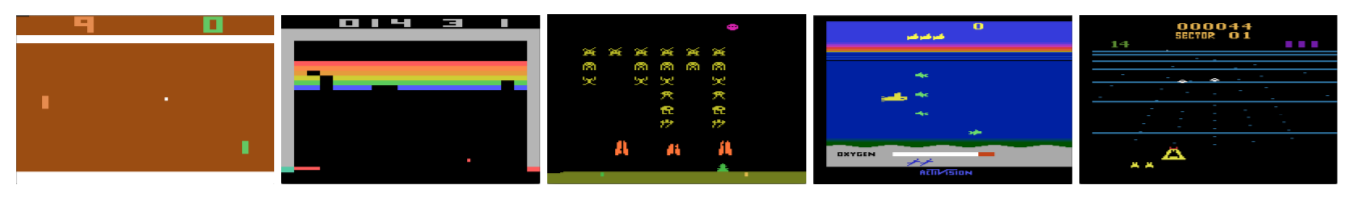
\includegraphics[keepaspectratio,
                     width=.85\paperwidth]{atari_games.png}

\hfill\hfill Pong \hfill  Breakout \  Space Invaders \  Seaquest \hfill Beam Rider
  \end{center}

  Состояния $s$: 4 последовательных кадра, сжатых до $84 \times 84$

  Действия $a$: от 4 до 18, в зависимости от игры

  Награды $r$: текущий SCORE в игре

  Функция ценности $Q(s, a; w)$: ConvNN со входом $s$ и $|A|$ выходами

  \noindent\rule{8cm}{0.4pt}

  {\small
  {\it V.Mnih et al.} (DeepMind). Playing Atari with deep reinforcement learning. 2013}

\end{frame}


\begin{frame}
  \frametitle{Метод DQN (Deep Q-Learning Network)}

  Сохранение траекторий $(s_t, a_t, r_t)_{t=1}^T$ в памяти (reply memory) для многократного воспроизведения опыта (experience replay)

  \vspace{0.2cm}
  Аппроксимация оптимальной функции ценности $Q(s_t, a_t)$ при фиксированных текущих параметрах сети ${\color{red} w_t}$

  $$ y_t =
  \left\{ \begin{aligned}
  &r_t, \text{ если состояние } s_{t+1} \text{ терминальное } \\
  &r_t + \gamma \max_a Q(s_{t+1}, a; {\color{red} w_t}), \text{ иначе}
  \end{aligned} \right.
  $$

  Функция потерь для обучения нейросетевой модели $Q(s, a; w)$:

  $$ \mathscr{L} (w) = (Q(s_t, a_t; w) - y_t)^2 $$

  Стохастический градиент SGD (по мини-батчам длины 32):

  $$ w_{t+1} = w_{t} - \eta \left(Q(s_t, a_t; w_t) - y_t\right) \nabla_w Q(s_t, a_t; w_t) $$
\end{frame}


\begin{frame}
  \frametitle{Архитектура сети для функции ценности}
  \begin{center}
    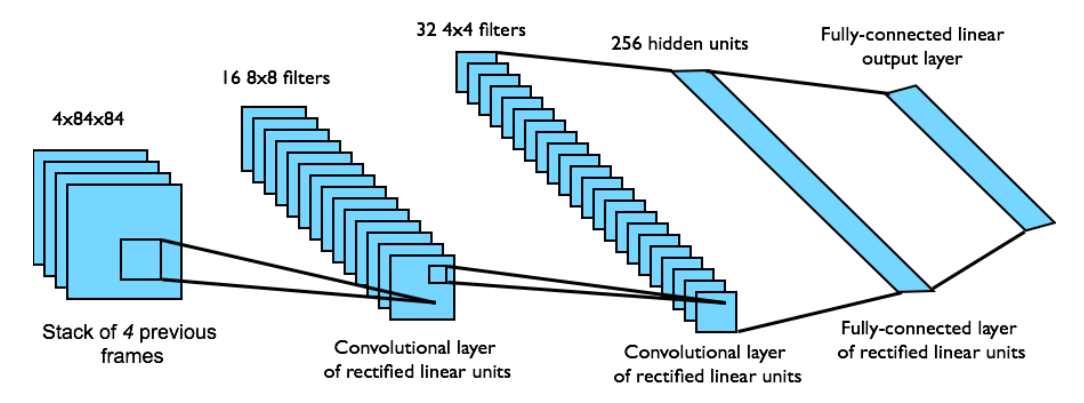
\includegraphics[keepaspectratio,
                     width=.85\paperwidth]{dql-cnn-arch.png}
  \end{center}
\end{frame}


{ % all template changes are local to this group.
    \setbeamertemplate{navigation symbols}{}
    \begin{frame}<article:0>[plain]
        \begin{tikzpicture}[remember picture,overlay]
            \node[at=(current page.center)] {
                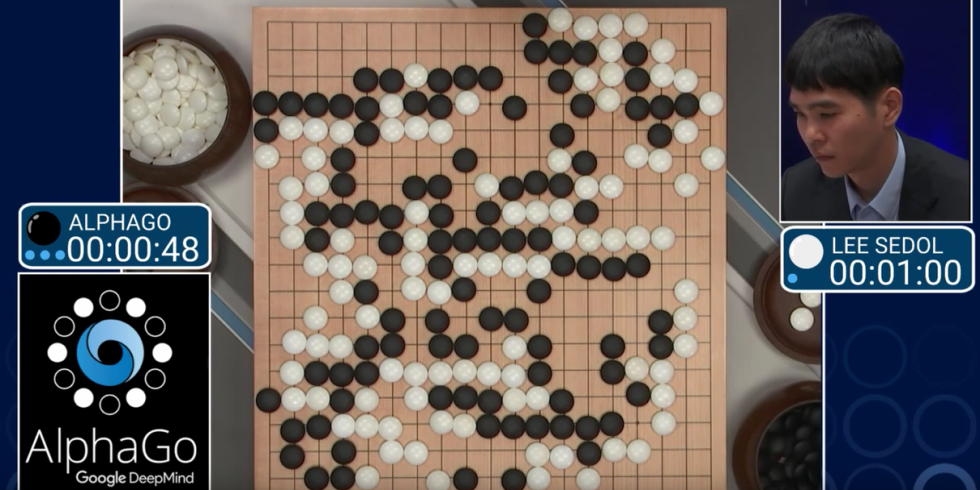
\includegraphics[keepaspectratio,
                                 width=\paperwidth,
                                 height=\paperheight]{alpha_go.png}
            };
        \end{tikzpicture}
     \end{frame}
}


{ % all template changes are local to this group.
    \setbeamertemplate{navigation symbols}{}
    \begin{frame}<article:0>[plain]
        \begin{tikzpicture}[remember picture,overlay]
            \node[at=(current page.center)] {
                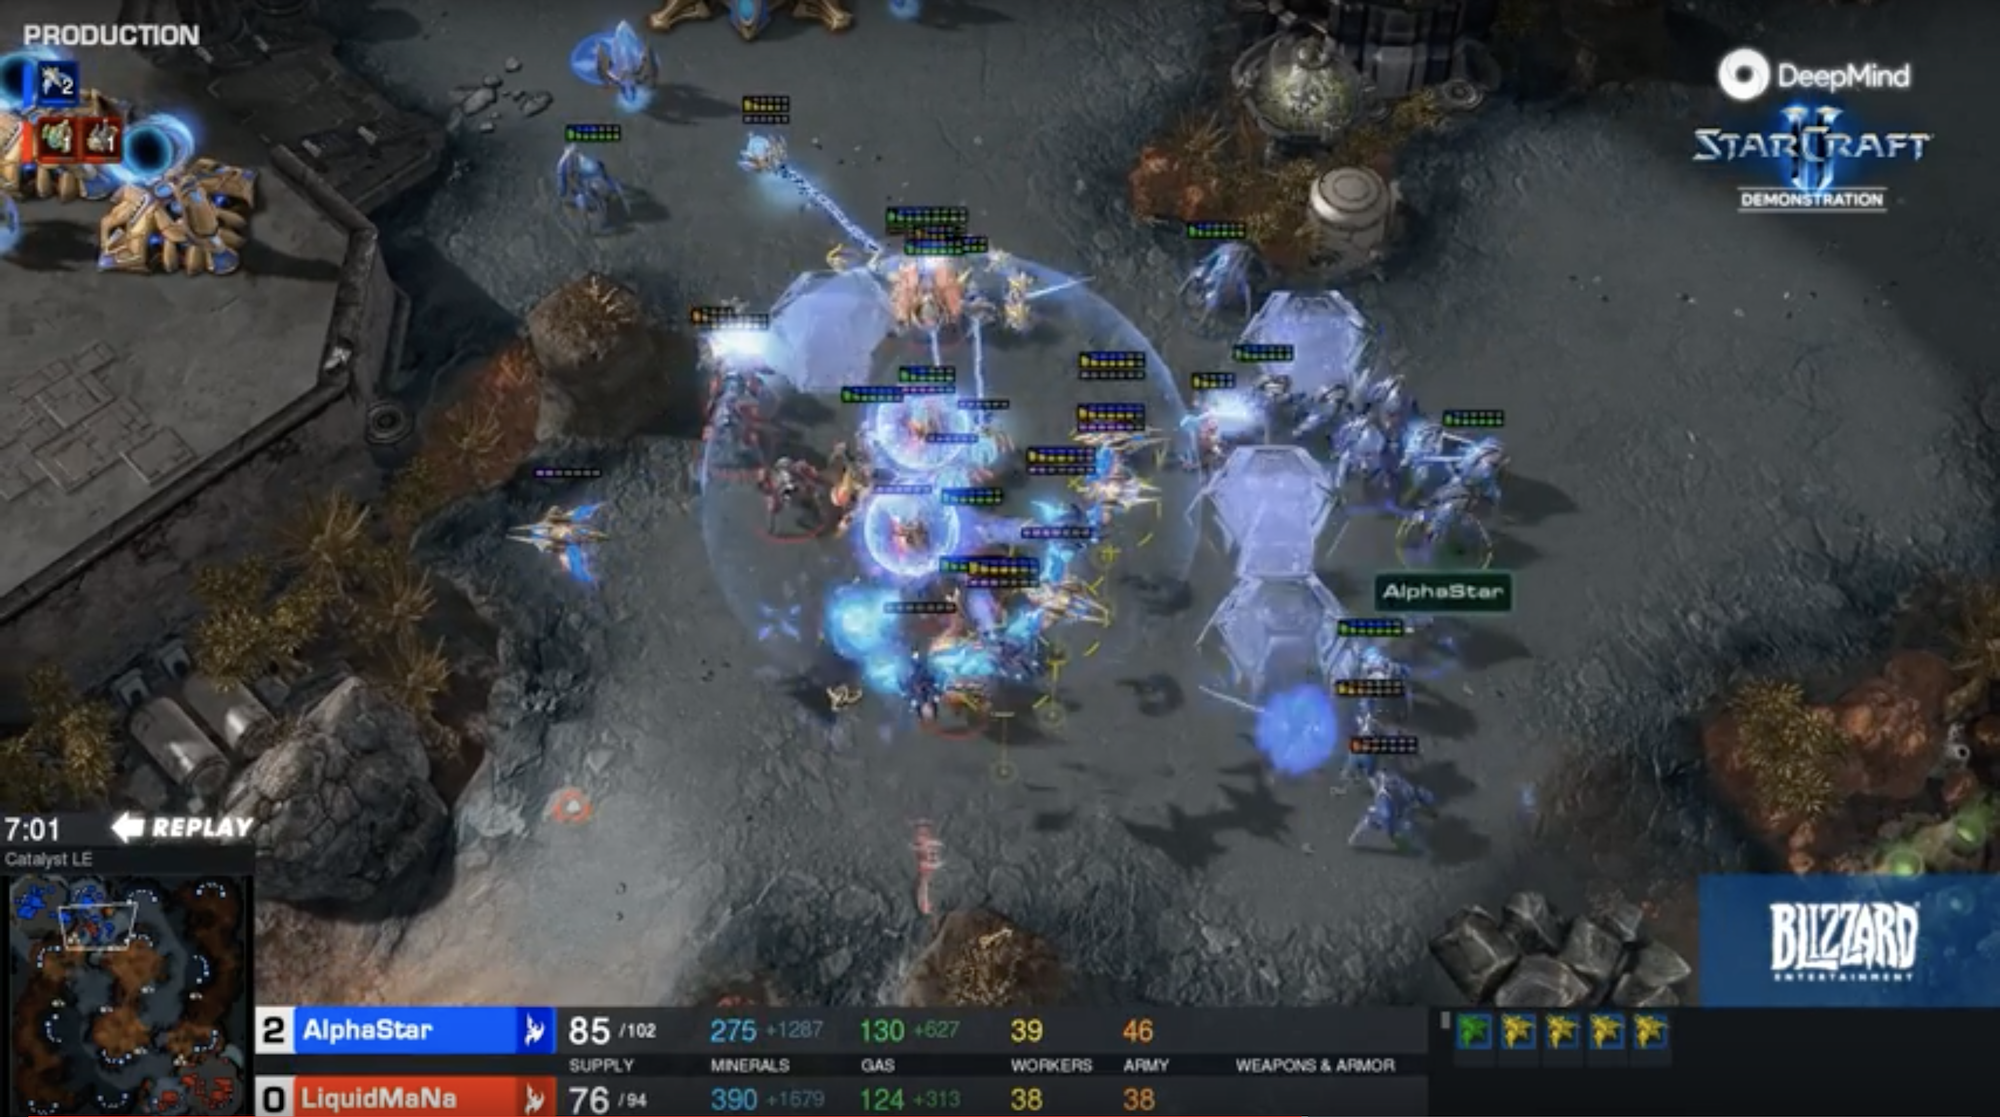
\includegraphics[keepaspectratio,
                                 width=\paperwidth,
                                 height=\paperheight]{AI-AlphaStar-StarCraft-II.png}
            };
        \end{tikzpicture}
     \end{frame}
}


\begin{frame}[t]
  \frametitle{Резюме}

  \begin{itemize}
    \item познакомились с постановкой задачи обучения с подкреплением
    \item вспомнили многоруких бандитов
    \item познакомились с методами кросс-энтропии, TD-обучения и Q-обучения
    \item обсудили Deep Q-learning Network
    \item НЕ обсудили центральный метод в роботике — градиентный спуск по стратегиям (policy gradient)
  \end{itemize}
  \vspace{0.5cm}
  \pause
  Что ещё можно посмотреть?

  \begin{itemize}
    \item главная книга по теме: \href{https://web.stanford.edu/class/psych209/Readings/SuttonBartoIPRLBook2ndEd.pdf}{Reinforcement Learning: An Introduction}, Richard S. Sutton and Andrew G. Barto
    \item \href{https://spinningup.openai.com/en/latest}{https://spinningup.openai.com/en/latest}
    \item Yuxi Li. Resources for Deep Reinforcement Learning. 2018
  \end{itemize}
\end{frame}

\end{document}
